\documentclass{article}
\usepackage[utf8]{inputenc}
\usepackage[margin=1in]{geometry}
\usepackage[colorlinks]{hyperref}
\usepackage{graphicx}
\usepackage{caption}
\usepackage{color}
\usepackage{subcaption}

\begin{document}
\title{\textbf{CS6011: Kernel Methods for Pattern Analysis}
\\
\textbf{Programming Assignment 1}
}
\author{Aravind Sankar CS11B033 \\
Ramnandan SK CS11B061 \\
Adit Krishnan CS11B063 \\[0.2in]
Group 2
}

\maketitle
\tableofcontents 

\section{Objective of the assignment}
The basic goal of this assignment is to use linear models of regression to do 2 Function Approximation tasks, namely Polynomial Curve fitting on Dataset 1 (univariate) and Surface Fitting using Gaussian Basis functions for Dataset 2 (bivariate). Here, the means of the Gaussians used are the centers of clusters obtained using K-means clustering of the training data. The experimental results obtained are to be summarized using plots obtained on varying different model parameters.
\section{Dataset 1}

\subsection{Generation}
The given function to be approximated is shown below :

\[ f(x) = e^{\cos(2 \pi x)} \]
\[ x \in (0,1) \]

\begin{flushleft}
To generate points from this function, we randomly generated points $x \in (0,1)$ and found the function value $f(x)$ at each point, and added to it Gaussian Noise with mean $\mu = 0$ and standard deviation $\sigma = 0.1$. 3 different training sets were generated, of sizes 20, 100 and 1000. The size of the validation and test set generated were 50 each.
\end{flushleft}

\subsection{Model creation}
\begin{flushleft}
As the goal is to fit a polynomial function to the given data, we need to decide on the degree $M$ of the polynomial which decides the model complexity. 

Through the plots, we show the variation of model outputs and RMS errors on varying different 
parameters and our analysis of the results to choose the best model.

\end{flushleft}

\subsection{Results}

\subsubsection{Plots of approximated functions}

Plots showing variation of the polynomial w.r.t degree of polynomial $M$, for training dataset of size $N = 20$. Each plot shows the data points \textcolor{green}{x}, the target function \textcolor{blue}{$f(x)$}  and the approximated polynomial \textcolor{red}{$y(x,\bar{w})$} 
\begin{figure}[hbtp]

\begin{subfigure}{.5\textwidth}
\centering
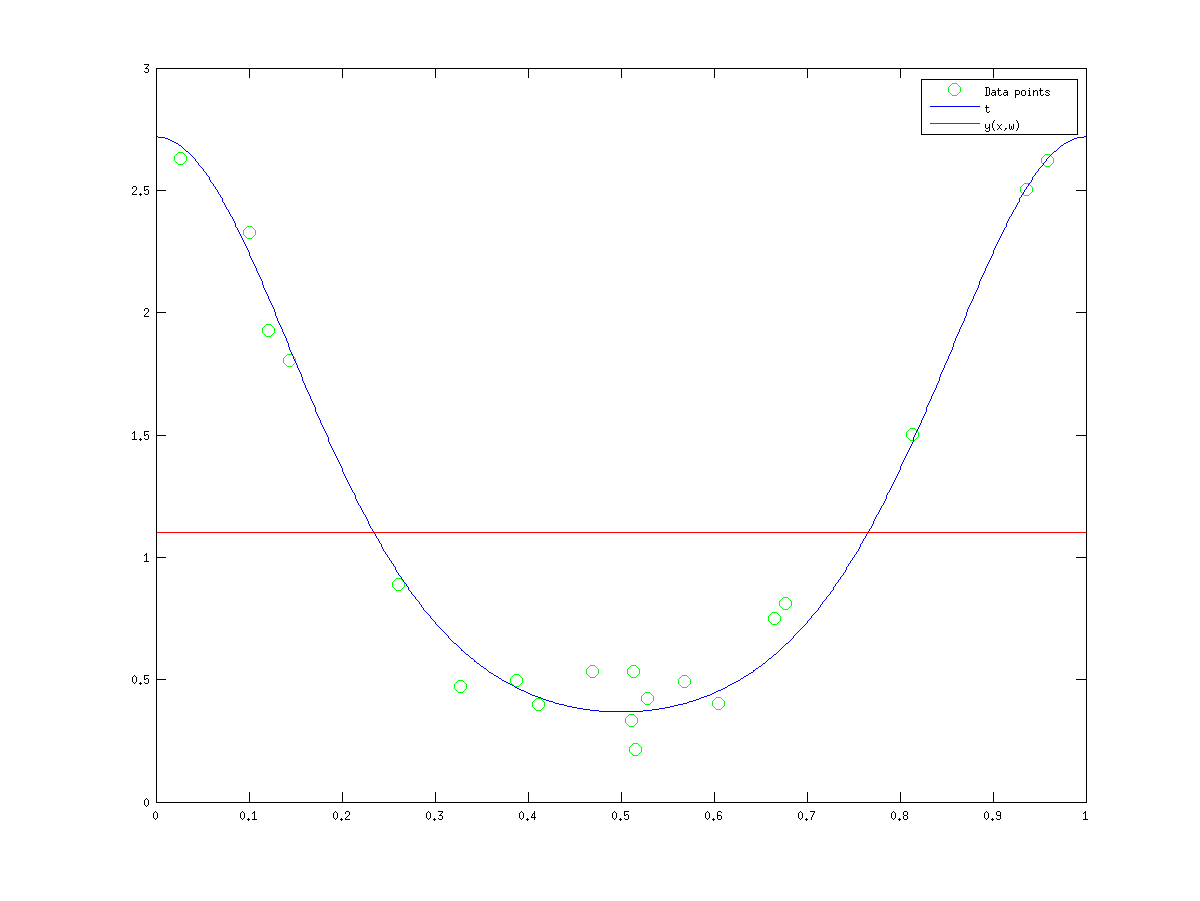
\includegraphics[width=\linewidth]{../Code/Plots_1/Varying_M/VaryingM_N20M0.png}
\caption{N = 20 M = 0}
\end{subfigure}
\begin{subfigure}{.5\textwidth}
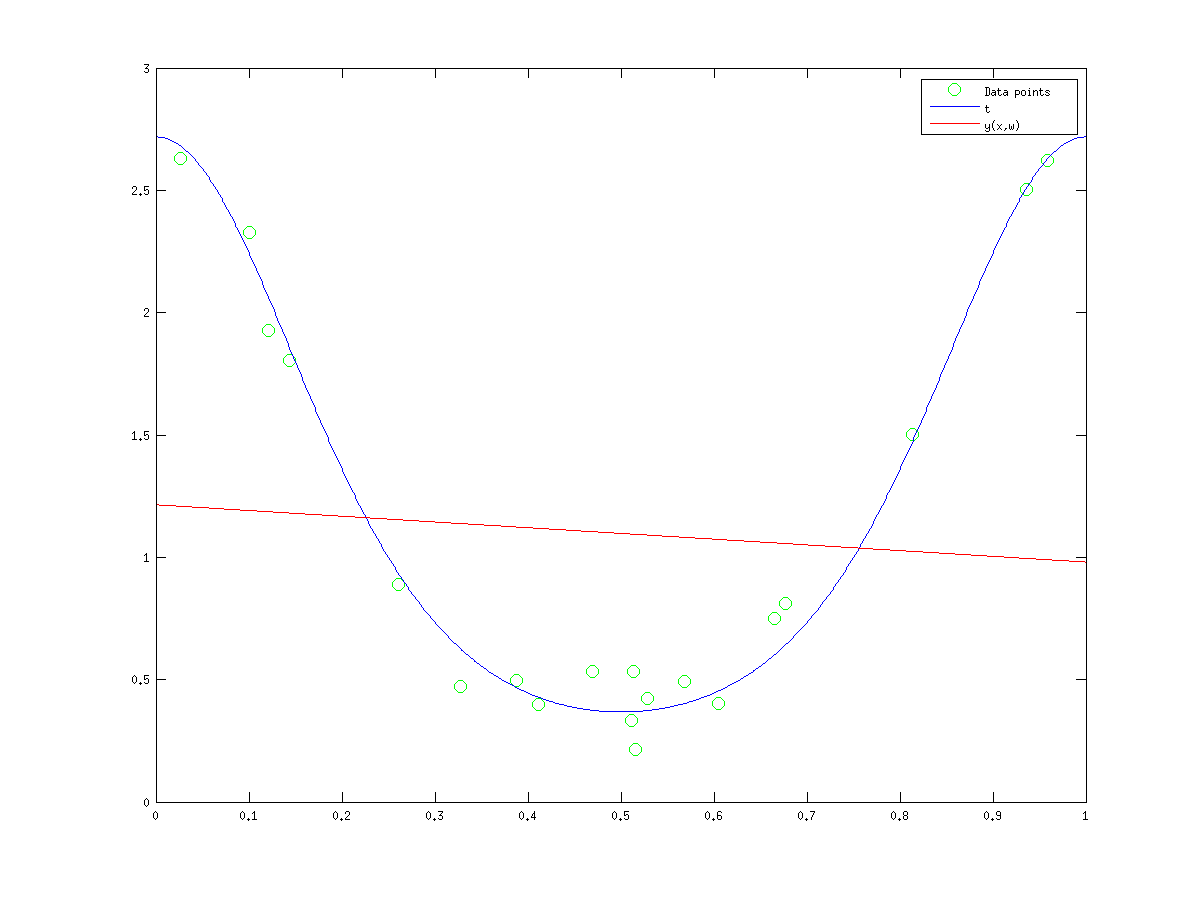
\includegraphics[width=\linewidth]{../Code/Plots_1/Varying_M/VaryingM_N20M1.png}
\caption{N = 20 M = 1}
\end{subfigure}


\begin{subfigure}{.5\textwidth}
\centering
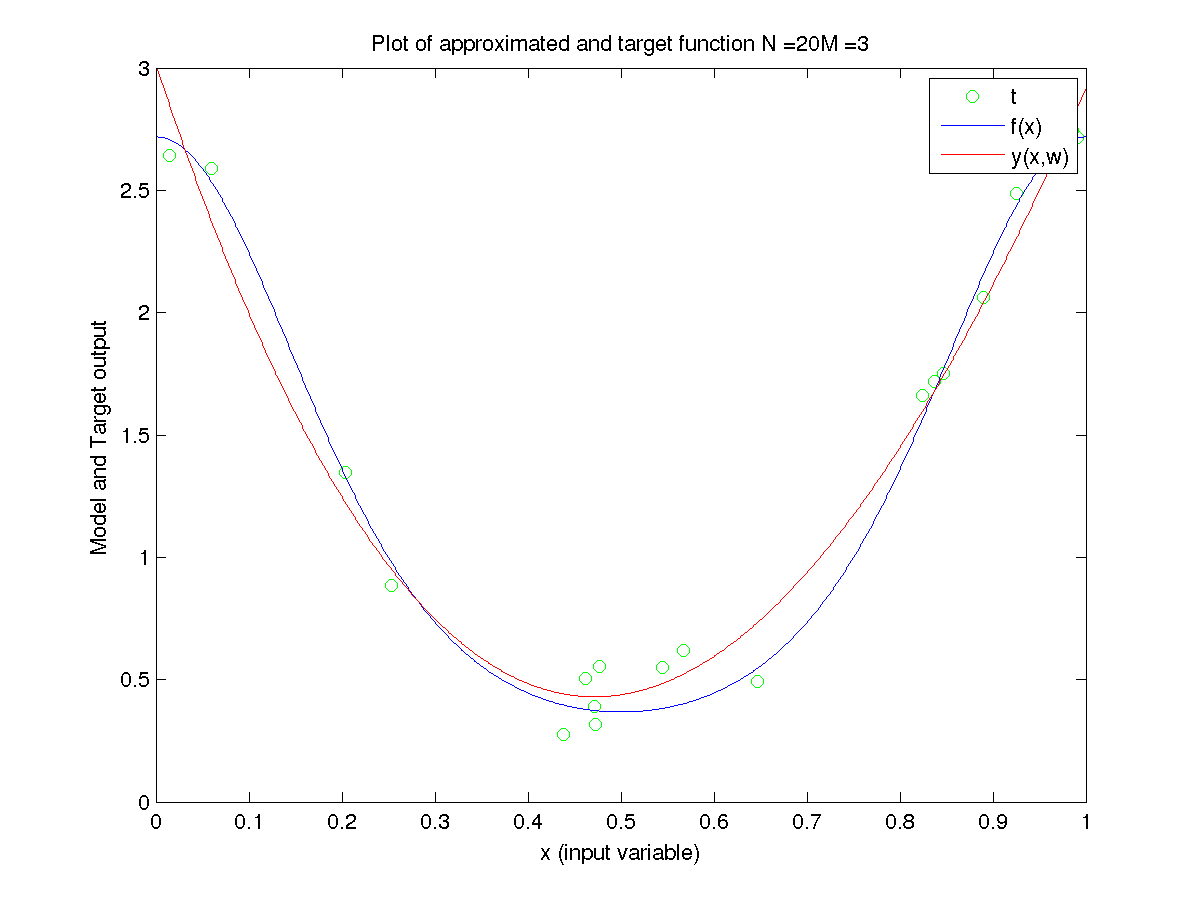
\includegraphics[width=\linewidth]{../Code/Plots_1/Varying_M/VaryingM_N20M3.png}
\caption{N = 20 M = 3}
\end{subfigure}
\begin{subfigure}{.5\textwidth}
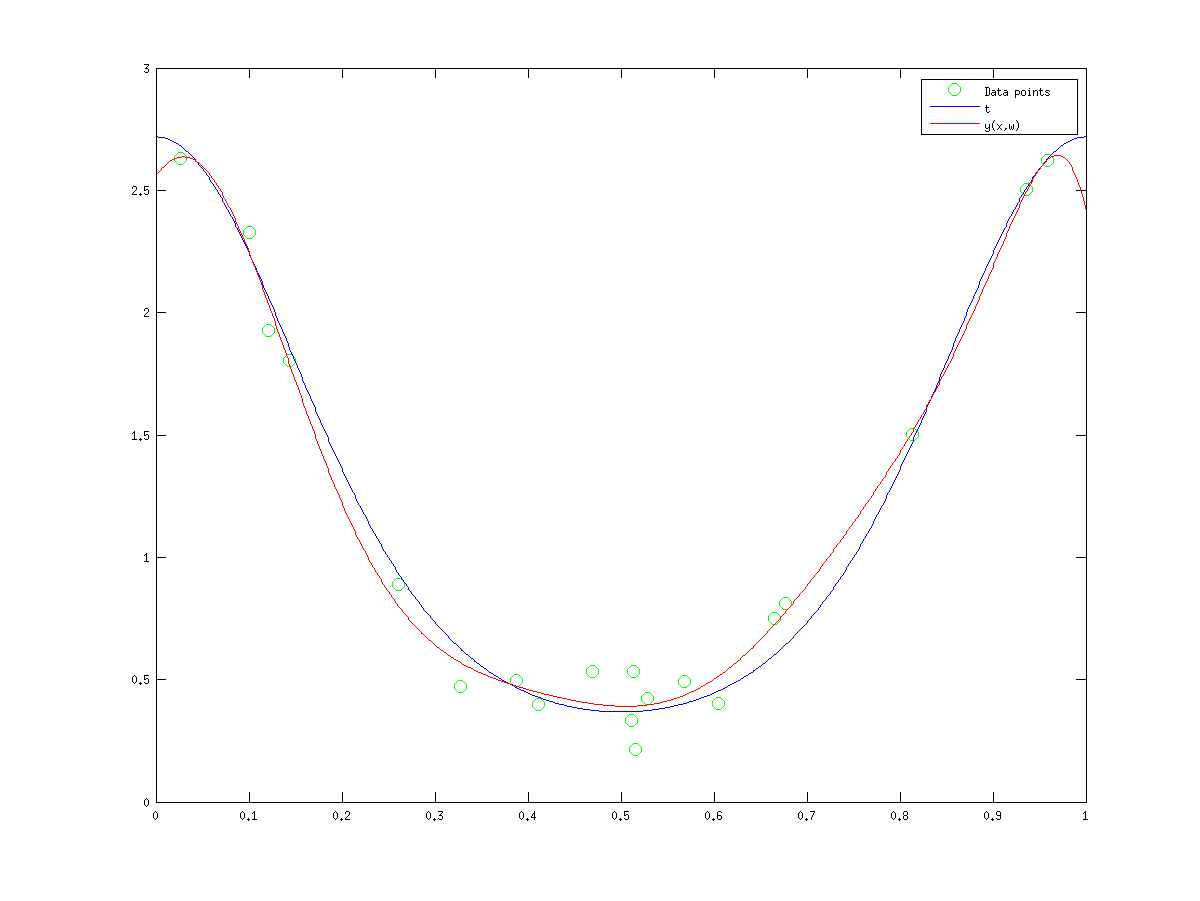
\includegraphics[width=\linewidth]{../Code/Plots_1/Varying_M/VaryingM_N20M9.png}
\caption{N = 20 M = 9}
\end{subfigure}



\end{figure}


The following plots show the different polynomials obtained on varying the training dataset size $N$. Each of these plots are shown for 2 values of $M$ - 9 and 15.


\section{Dataset 2}

\subsection{Generation}

\subsection{Model creation}
\subsection{Results}

\subsection{Plots of approximated functions}


\end{document}
